\documentclass[final]{svjour2}
\usepackage{graphicx}
\usepackage{rotating}
\usepackage{amssymb}
\usepackage{mathptmx}
\usepackage[numbers]{natbib}
\usepackage{float}
\usepackage[section]{placeins}
%\usepackage[nofighead,nomarkers]{endfloat}
\makeatletter
\journalname{Journal of Low Temperature Physics}
%%%%%%%%%%%%%%%%%%%%%%%%%%%%%% Textclass specific LaTeX commands.
%%%%%%%%%%%%%%%%%%%%%%%%%%%%%% User specified LaTeX commands.
\bibpunct{}{}{,}{s}{}{,}

\begin{document}

\newcommand{\hdblarrow}{H\makebox[0.9ex][l]{$\downdownarrows$}-}
\title{Design Considerations for Cryogenic Support Structures}

\author{E. Kramer \and N. Kellaris  \and M. Daal \and N. Zobrist \and S. Govindjee \and B. Sadoulet \and S. Golwala \and M. Hollister}

\institute{Department of Physics, U.C. Berkeley,\\ Berkeley, CA 94709, USA\\
\email{ekramer@berkeley.edu}}

\date{07.15.2013}

\maketitle

\begin{abstract}

Design specifications for the support structures of low temperature instrumentation often call for low thermal conductivity between temperature stages, high stiffness and defined load bearing capabilities.  The challenge is usually to find a design that minimizes heat transfer while meeting strength and rigidity specifications.  Common design solutions employ thin-walled tubes and truss structures. In this contribution, we suggest, analyze and test several design solutions that incorporate such structures. In addition, we present some equations for failure modes and structural stiffness.

\keywords{Truss, Thin-walled tube, Cryogenic Tower}

\end{abstract}

\section{Introduction}
Both slender member truss and thin-walled tube structures exhibit desirable qualities for low temperature instrumentation support structures due to their high structural stiffness to low thermal conductivity across stages.  Designing optimal structures that obtain the least amount of thermal loss between stages while still remaining structurally adequate to support both forces while in use and handling is a processes of optimization.  Theoretical equations and computer simulation of structural stiffness allow one narrow down possible design choices without needing to fabricate and physically test each design iteration.  While highly useful, calculations and computer simulations are not sufficient on their own. In the lab under non-ideal circumstances, materials and designs typically fail before their theoretical failure point due to imperfections, including but not limited to impurities in the material, microscopic fractures or hole, and misaligned or misshapen elements of the overall design.  Due to this, physical strength testing of a fabricated piece can be performed to confirm failure modes as well as discover unexpected ones.  Results from such tests allow one to better obtain the performance and factor of safety desired for the part being designed.

\section{Experimental details}
For this experiment, we began with theoretical analysis via computer simulation and then proceeded to fabricate and physically test a few promising designs.  Our truss structure analysis was performed using the method of joints as basis.  In this technique the forces at each node were statically determined while taking into account the boundary conditions (fixed, clamped, free), connectivity, and external loading.  This method allows us to solve for all the forces along each truss member as well as all of the reaction forces on the fixed pin joints for any given stable structure.  Using these solutions and the material properties of the truss members failure points were identified for each member, giving the structure an overall point of failure at when its weakest member fails.  Tube analysis was done using the equations presented by Govindjee in (BIB REFERENCE HERE)

(INSERT GOVINDJEE EUQUATIONS HERE)

Using these theoretical results, we then fabricated a few promising designs, including a hexapod truss structure and several pure thin walled tubes. 

\begin{figure}[!ht]
\begin{center}
\includegraphics[%
  width=0.9\linewidth,
  keepaspectratio]{SW}
\end{center}
\caption{Our hexapod truss design (left) and a simple thin-walled tube design (right). Not to scale.}
\label{SW}
\end{figure}

These fabricated parts were then subjected to a variety of loads on an (MACHINE TYPE NAME?) to compare the results to the theoretical ones found previously.  Strength testing was done on a single axis machine with tension and compression capabilities. Samples were fitted to be able to be locked into the machine both along their center axis as well slightly off axis in order to test both tensile and compressive strength in the on axis and off axis.  An external frame was also used to allow our samples to be mounted horizontally, either supported as a pair of cantilever beams or a single simply supported beam, to be tested for pure shear and bending stiffness respectively.  We tested four sample types consisting of three truss structures and one thin-walled tube structure.  All three truss structures were identical in overall design, utilizing six members to connect two copper or aluminum hexagons base plates.  We tested three different types of truss members which included two Graphlite of 40 and 80 mil cross sectional diameters and one Titanium rectangular cross section member. The thin-walled tube structures were constructed from a single two inch length of two inch outside diameter Vespel tube connected with Stycast 1266 to two gold-plated copper baseplates. Two SP1 and SP22 10 mil wall thickness truss tube members were also fabricated to test on their own.

\begin{figure}[!ht]
\begin{center}
\includegraphics[%
  width=0.9\linewidth,
  keepaspectratio]{fab}
\end{center}
\caption{Fabricated tube supports (right) and hexapod truss structures utilzing both 40 mil and 80 mil Graphlite members (left)}
\label{fab}
\end{figure}

\section{Results}
Currently simulation and testing has been completed on the 40 and 80 mil truss structures under a pure bending load and on the SP1 and SP22 tubes in tension.  All samples were tested to failure in a strain controlled environment.  The pull rate was 0.5 mm/sec for all tests.  Results of the four tests in a plot of stress vs strain is presented below.

\begin{figure}[!ht]
\begin{center}
\includegraphics[%
  width=0.65\linewidth,
  keepaspectratio]{Test}
\end{center}
\caption{The stress and strain vs time of four strength tests. 40 mil Graphlite hexapod in pure bending (top-left), 80 mil Graphlite hexapod in pure bending (top-right), 10 mil wall thickness SP1 tube truss member in tension (bottom-left), and 10 mil wall thickness SP22 tube truss member in tension (bottom-right).}
\label{Test}
\end{figure}
(Discussion of strength test results? Compare to Matt's? or Erik's? Present theoretical data?)

\section{Design Considerations and Material Selection}
When designing truss and tube structures there are a multitude of design choices available to meet the constraints of the system.  Material type, truss member cross-section, tube wall thickness, and overall structure layout are all variables that can be set by the designer.  Each of these variables add degrees of freedom to designing, making it difficult to have a single recipe for the optimum structure.  There are certain design considerations however that can lead to stiffer and more predictable structures.  Buckling is a major concern when using slender truss members.  While not always resulting in fracture of the structure, it can have a fast onset and lead to a severely deformed structure.  When choosing materials, one should note that buckling tends to occur before other failure modes in non-brittle materials. The use of tubes as truss members reduces the susceptibility to buckling due to the fact that buckling is a more prominent failure mode in solid rods.  While not ideal for truss structures in terms of theoretical functionality, clamping joints as opposed to letting them be free to rotate reduces susceptibility to buckling thus giving the overall structure greater stiffness. Also when designing trusses, placing the joints in line with the connecting members offers the greatest stability due to truss members ideally only carry forces along their normal direction.  Symmetry should be noted as well when designing as any type of non symmetrical structure can fail in a non-symmetrical way.  Finally holes or other surface features of any type should be avoided whenever possible because they will result in stress concentrations of several factors which in turn leads to earlier failure.  

Along with design choices themselves, material selection is also an important  choice in both thin-walled tubes and truss structures. Youngs Modulus is a material specific property that directly defines a materials stiffness or elasticity.  Materials with high Youngs Modulus are better suited for creating stiff structures. Materials cannot be solely selected on their structural properties however, as thermal resistivity is also a concern in cryogenic support structures.  Materials must be stiff enough to not fail under expected loads ranges while keeping their cross section is low as possible to minimize the amount of heat transfer between temperature stages.  In general when choosing materials we desire the smallest Thermal conductivity to Youngs Modulus ratio.  The plot below we present a few useful materials with a low thermal conductance to Youngs Modulus ratio.

\begin{figure}[!ht]
\begin{center}
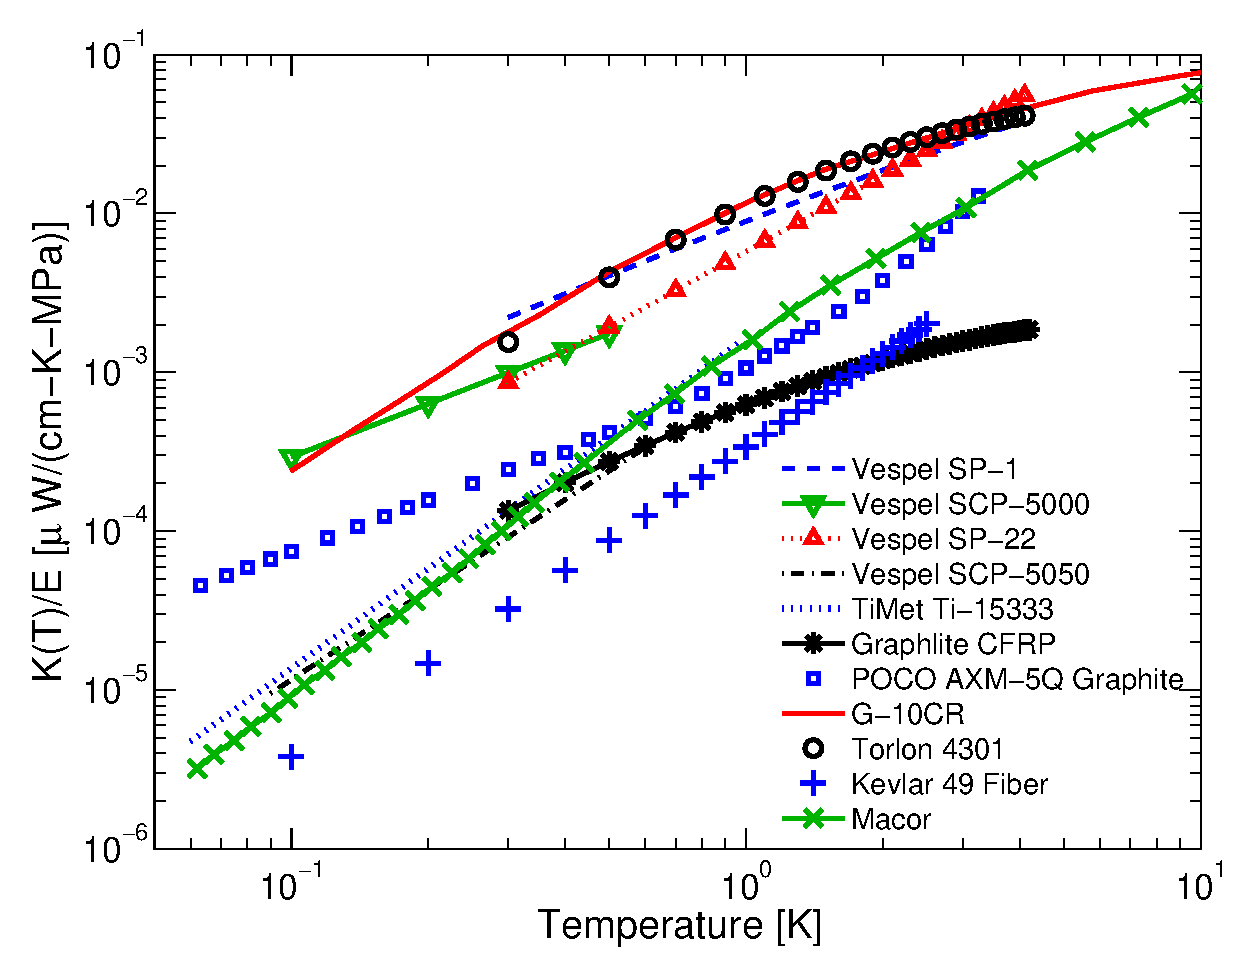
\includegraphics[%
  width=0.65\linewidth,
  keepaspectratio]{Mats}
\end{center}
\caption{A selections of materials with their Youngs modulus normalized by their thermal conductivity.  Lower values correspond to more ideal materials for support structures}
\label{Mats}
\end{figure}

\section{Conclusions}
While many different solutions are available when creating cryogenic support structures, following certain design criteria and avoiding potential pitfalls that compromise structural strength allow for tube and truss structures to remain string while providing low heat loads between stages.  It is important to design with a large factor of safety beyond the theoretical failure point of a structure due to the imperfection dominated failure modes that exist in actual structures of this variety.  When considering truss members, tubes offer high stiffness but little to no elastic region before fracture.  Rods offer more elasticity which makes them susceptible to buckling.

\begin{acknowledgements}
We would like to thank S. Govindjee for technical assistance and use of his strength testing equipment. We acknowledge support and funding from the Department of Energy and the National Science Foundation.
\end{acknowledgements}

\begin{thebibliography}{99}

\bibitem{Govindjee}
Govindjee paper (FINISH THIS)

\bibitem{Hastings}
Hastings paper (FINISH THIS)

\end{thebibliography}

\end{document}
